\documentclass[10pt,a4paper]{beamer}

\usepackage[utf8]{inputenc}
\usepackage[russian]{babel}
\usepackage[OT1]{fontenc}
\usepackage{amsmath}
\usepackage{amsfonts}
\usepackage{amssymb}
\usepackage{makeidx}
\usepackage{graphicx}
\usepackage{xcolor}
\usepackage{multirow}
\usepackage{framed}
\definecolor{shadecolor}{cmyk}{0,0,0,1}
\usepackage{hyperref}
\usepackage[normalem]{ulem}

\titlegraphic{
   
\includegraphics[width=4cm]{images/sfera.jpg}
}

\author{Николай Анохин \and Михаил Фирулик}
\title{Введение в Data Science \\ Занятие 7. Ноунейм}

\beamertemplatenavigationsymbolsempty

\begin{document}

\maketitle

\logo{
    
\includegraphics[width=4cm,keepaspectratio]{images/sfera.jpg}\hspace{0.45em}
}

% ============================================== %

\begin{frame}{Работа в группе}

{\bf Задача.} Оценить, какой вклад внес в общий результат каждый участник группы

\vspace{1em}
{\bf Шаг 1.} Каждый студент {\bf анонимно и независимо} распределяет 100 очков между всеми участниками своей группы в зависимости того, какую пользу (по его/её мнению) каждый из участников принес

\vspace{1em}
{\bf Пример.}

\begin{center}
\begin{tabular}{l c}
Студент & Вклад \\
\hline
Геральт & 50 \\
Лютик & 10 \\
Мильва & 20 \\
Регис & 20
\end{tabular}
\end{center}

{\bf Шаг 2.} Из всех оценок вычисляется общая аггрегированная оценка на основе алгоритма PageRank

\end{frame}

% ============================================== %

\begin{frame}{План занятия}

\tableofcontents

\end{frame}

% ============================================== %

\section{PageRank}

% ============================================== %

\begin{frame}{Жизнь до Google}

\begin{center}

\end{center}
\vspace{-2em}
\begin{columns}[C]
    \begin{column}{.55\textwidth}
    \begin{enumerate}    
	\item Поисковые роботы используются для парсинга интернет-страниц
	\item Составляется обратный индекс, в котором каждому слову соответствовал  набор страниц
	\item Слова из поискового запроса пользователя используются для поиска страниц в индексе
	\item Из {\bf близких} к запросу страниц формируется выдача
	\end{enumerate}
	\vspace{1em}
	{\it \hspace{3em}Проблема: Term Spam}
    \end{column}
    \begin{column}{.55\textwidth}
    
\includegraphics[scale=0.24]{images/lantern.png}
	\end{column}
\end{columns}

\end{frame}

% ============================================== %

\begin{frame}{Что придумали парни из Google}

\begin{columns}[C]
	\begin{column}{.50\textwidth}
    \vspace{1em}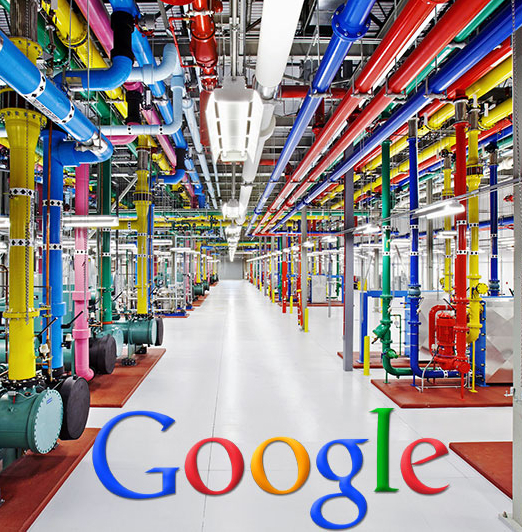
\includegraphics[scale=0.30]{images/google.jpg}
	\end{column}
    \begin{column}{.5\textwidth}
    \hspace{1em}Дополнительно
    \begin{enumerate}    
	\item Страницы ранжируются в соответствии с их ``важностью'' с помощью алгоритма PageRank
	\item О релевантности страниц судят не только по словам, находящимся на текущей странице, но и по словам ``соседних'' страниц
	\end{enumerate}
    \end{column}
\end{columns}

\end{frame}

% ============================================== %

\begin{frame}{Random Surfer}

\begin{block}{Интуиция}
Пользователь начинает с просмотра случайной страницы, после чего с равной вероятностью переходит по одной из ссылок на этой странице. Процесс продолжается до бесконечности. PageRank страницы -- вероятность обнаружить пользователя на этой странице.
\end{block}

\begin{itemize}
\item Пользователь с большей вероятностью посещает ``полезные'' страницы, чем ``бесполезные''
\item Создатели страниц размещают ссылки на ``полезные'' страницы
\end{itemize}

\end{frame}

% ============================================== %

\begin{frame}{PageRank}

Представим интернет, как направленный граф со страницами в качестве вершин и ссылками между страницами в качестве ребер

\vspace{2em}
\begin{columns}[C]
	\begin{column}{.5\textwidth}
    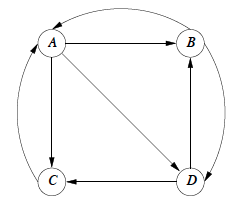
\includegraphics[scale=0.60]{images/pr1.png}
	\end{column}
    \begin{column}{.5\textwidth}
    Матрица вероятностей перехода
    \[
    M = \begin{pmatrix}
    0 & 1/2 & 1 & 0 \\
    1/3 & 0 & 0 & 1/2 \\
    1/3 & 0 & 0 & 1/2 \\
    1/3 & 1/2 & 0 & 0 \\
    \end{pmatrix}
    \]        
    \end{column}    
\end{columns}

\end{frame}

% ============================================== %

\begin{frame}{PageRank}

\begin{columns}[C]
	\begin{column}{.5\textwidth}
    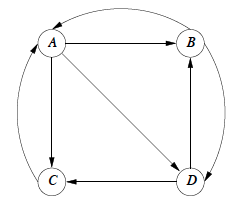
\includegraphics[scale=0.60]{images/pr1.png}
	\end{column}
    \begin{column}{.5\textwidth}
    Элементы матрицы перехода
	\[
	m_{ij} = P(\mathbf{v}_i^{(k)} | \mathbf{v}_j^{(k-1)})
	\]
	Изначально все страницы равновероятны
	\[
	\mathbf{v}^{(0)} = \begin{pmatrix}
	1/n & \ldots & 1/n
	\end{pmatrix}^\top
	\]
	Вектор вероятностей на $k$ шаге
	\[
	\mathbf{v}^{(k)} = M \mathbf{v}^{(k-1)}
	\]
    \end{column}
    
\end{columns}

\vspace{2em}
Предельное значение $\mathbf{v}$ -- собственный вектор $M$, соответствующий собственному числу $\lambda=1$. Процесс сходится, если из любой вершины можно попасть в любую.

\end{frame}

% ============================================== %

\begin{frame}{Структура Интернета}

\begin{center}
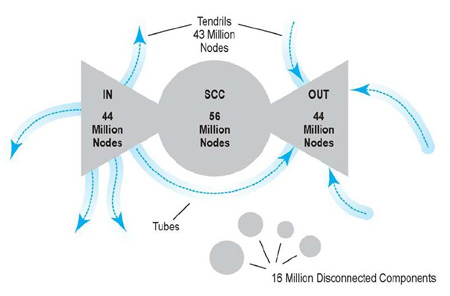
\includegraphics[scale=0.65]{images/internet.jpg}
\end{center}

\end{frame}

% ============================================== %

\begin{frame}{Проблемы PageRank}

\begin{columns}[T]
	\begin{column}{.5\textwidth}
	\hspace{7em}Dead End	
    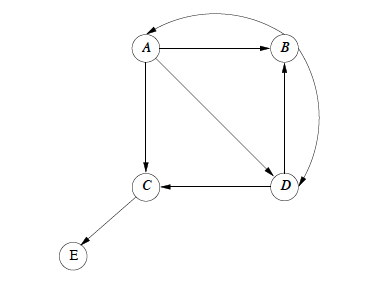
\includegraphics[scale=0.45]{images/de.png}
	\end{column}
    \begin{column}{.5\textwidth}
    \hspace{5em}Spider Trap
	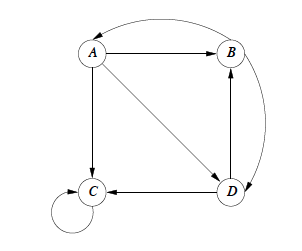
\includegraphics[scale=0.45]{images/st.png}
    \end{column}    
\end{columns}

{\bf Решение.} разрешим пользовалю ``телепортироваться'' на случайную страницу с вероятностью $1 - \beta$
\[
\mathbf{v}^{(k)} = \beta M \mathbf{v}^{(k-1)} + (1 - \beta) \frac{\mathbf{e}}{n} 
\]

\end{frame}

% ============================================== %

\begin{frame}{Пример}

\begin{columns}[C]
	\begin{column}{.5\textwidth}
	Матрица перехода
 \[
    M = \begin{pmatrix}
    0 & 1/2 & 0 & 0 \\
    1/3 & 0 & 0 & 1/2 \\
    1/3 & 0 & 1 & 1/2 \\
    1/3 & 1/2 & 0 & 0 \\
    \end{pmatrix}
 \] 
Без телепортов
\[
\mathbf{v} = \begin{pmatrix}
0 & 0 & 1 & 0
\end{pmatrix}
\]
С телепортами $\beta = 0.8$
\[
\mathbf{v} = \begin{pmatrix}
\frac{15}{148} & \frac{19}{148} & \frac{95}{148} & \frac{19}{148}
\end{pmatrix}
\]
	\end{column}
    \begin{column}{.5\textwidth}
    \hspace{5em}Spider Trap
	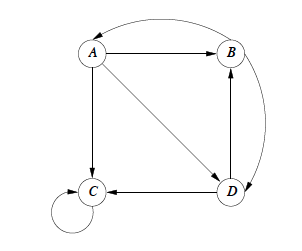
\includegraphics[scale=0.45]{images/st.png}
    \end{column}    
\end{columns}

\end{frame}

% ============================================== %

\begin{frame}{Методика оценки}

\begin{center}
\begin{tabular}{l | c c c c | c}
 & Геральт & Лютик & Мильва & Регис & Индивидуально \\
\hline
Геральт & 50 & 10 & 30 & 30 & 20\\
Лютик & 10 & 70 & 10 & 5  & 5\\
Мильва & 20 & 10 & 30 & 30 & 15\\
Регис & 20 & 10 & 30 & 35 & 15
\end{tabular}
\end{center}

Матрица перехода, $\beta=0.9$ 
\[
M = \begin{pmatrix}
0.5 & 0.1 & 0.3 & 0.3 \\
0.1 & 0.7 & 0.1 & 0.05 \\
0.2 & 0.1 & 0.3 & 0.3 \\
0.2 & 0.1 & 0.3 & 0.35
\end{pmatrix} \quad
v = \begin{pmatrix}
0.31 \\
0.23 \\
0.23 \\
0.24
\end{pmatrix}
\]
Групповая оценка: 30/40

\vspace{1em}
{\bf Итог:} \\ 
Геральт: 29, Лютик: 12, Мильва: 22, Регис: 22

\end{frame}

% ============================================== %

\end{document}